\documentclass[11pt]{scrreport}
\usepackage[utf8]{inputenc}
\usepackage{lmodern}
\usepackage[english] {babel}
\usepackage[T1]{fontenc}
\usepackage{graphicx,float}
\usepackage{booktabs}
\usepackage{amsfonts}
\usepackage{amsmath}
\usepackage[dvipsnames]{xcolor}
\usepackage{suffix}
\usepackage{xstring}
\usepackage[onehalfspacing]{setspace}
\usepackage{chemformula}
\usepackage[breaklinks,pdfpagelabels,hidelinks]{hyperref}%
\usepackage[figure]{hypcap}
\usepackage{cleveref}
\usepackage[style=chem-angew, backend=biber,doi,chaptertitle,articletitle]{biblatex}
\usepackage{chemfig}
\usepackage[right=2.5cm, left=2.5cm, top=2.5cm, bottom=2.5cm]{geometry}%,showframe
\usepackage{ragged2e}
\usepackage{caption}
\usepackage[section]{placeins}
\usepackage{colortbl}
\usepackage{float}
\usepackage{mathtools}
\usepackage{multirow}
\usepackage{siunitx}
\sisetup{detect-all}
\usepackage[useregional]{datetime2}
\usepackage[nopostdot,style=super,acronyms,nonumberlist,toc,translate=babel]{glossaries-extra}
\usepackage{tikz}
\usepackage{csquotes}
\usepackage[list=true]{subcaption}
\setcounter{tocdepth}{4}
\setcounter{secnumdepth}{4}
\renewcommand{\familydefault}{\sfdefault}
\addbibresource{SoftMatter.bib}
\let\cite=\supercite
\numberwithin{equation}{chapter}
%\addto{\captionsgerman}{\renewcommand*{\contentsname}{Inhaltsverzeichnis}}


\DefineBibliographyExtras{english}{%
	\DeclareBibstringSet{latin}{andothers,ibidem}%
	\DeclareBibstringSetFormat{latin}{\mkbibemph{#1}}%
}
\UndefineBibliographyExtras{english}{%
	\UndeclareBibstringSet{latin}%
}
\DefineBibliographyStrings{english}{%
	andothers = {et al\adddot},
}
\renewcommand\mkbibnamefamily[1]{\textsc{#1}}
\raggedbottom
\begin{document}
	\begin{titlepage}
		\setcounter{page}{0}
		\centering
		\includegraphics[width=0.6\textwidth]{"HHU_Logo_WortBildMarke.png"} 
		\vfill
		{\LARGE\bfseries Lab report: \\4. Synthesis of poly(N-isopropylacrylamide)-co-methacrylic acid microgels via precipitation} \\
		\vfill
		Faculty of Mathematics and Natural Sciences\\
		Heinrich Heine-University Düsseldorf\\
		\vfill
		for the module\\
		Soft Matter\\
		Advanced Materials (AdMat)\\
		in the sommer semester 2026
		\vfill
		Supervising assistant: Se\c{c}kin Altuncu\\
		Date of submission: \today
		\vfill
		by:\\
		\begin{tabular}{cc}
			Lena-Marie Aßmann    &  Nils Wölke\\
			\href{mailto:lena-marie.assmann@hhu.de}{lena-marie.assmann@hhu.de}    & \href{mailto:nils.woelke@hhu.de}{nils.woelke@hhu.de} 
		\end{tabular}
		\vfill
	\end{titlepage}
	\pagenumbering{Roman}
	\setcounter{page}{1}
	\tableofcontents
	\newpage
	\pagenumbering{arabic}
	\chapter{Introduction}
	Within this experiment a microgel consisting of statistical copolymers of N-isopropylacrylamide\linebreak (NIPAM) and methacrylic acid (MAA) with N,N-methylene(bis)acrylamide (MBA) as a crosslinker were to be synthesised via precipitation polymerization. The influence on the zeta potential was to be observerd by variation of the MA amounts.
	{\let\clearpage\relax\chapter{Theoretical Background}}
	\section{Microgels}
	Microgels are defined as \SIrange{0.1}{100}{\micro\meter} gel particles of in equivalent diameter in any shape, where a gel is defined as a three-dimensional polymer network swollen by a solvent. Due to their architecture unique properties can be observed, such as their softness and therefore deformability, or conformation change in different solvents.\cite{noauthor_microgel_2025,karg_nanogels_2019}\\
	As depicted in \autoref{fig:Microgel_synthesis} the synthesis of microgels happens in multiple steps. In a radical polymerization, oligoradicals form and assemble and grow to particles. \cite{klinger_stimuli-responsive_2012}
	\begin{figure}[H]
		\centering
		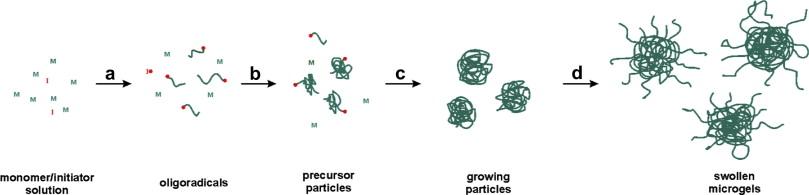
\includegraphics[width=\textwidth]{Microgel_synthesis.JPG}
		\caption{General mechanism for the formation of microgels during the synthesis in precipitation polymerization. Taken from \citeauthor{klinger_stimuli-responsive_2012} (\citedate{klinger_stimuli-responsive_2012}).\cite{klinger_stimuli-responsive_2012}}
		\label{fig:Microgel_synthesis}
	\end{figure}\noindent
	By lowering the temperature underneath the volume phase transition temperature (VPTT) the particles become swollen microgels. The VPTT is the temperature where swelling and deswelling by expelling or absorbing solvent occurs.\cite{klinger_stimuli-responsive_2012}
	\begin{figure}[H]
		\centering
		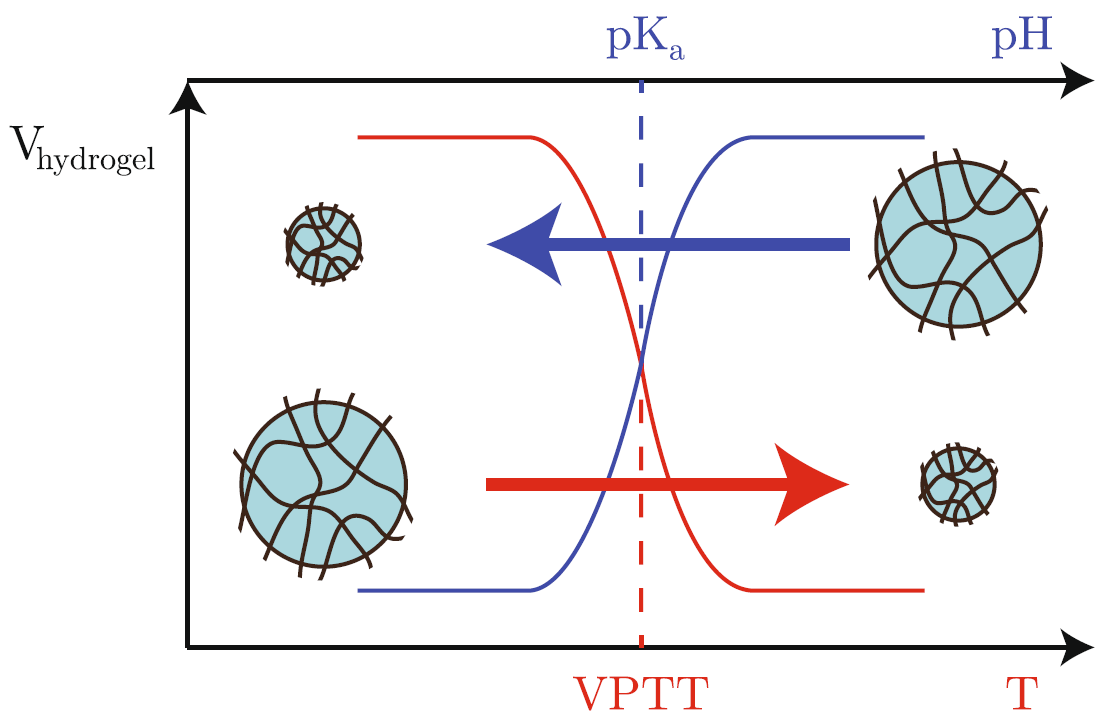
\includegraphics[width=0.5\textwidth]{Microgel_VPTT.PNG}
		\caption{Schematic illustration of the effect of temperature and pH on microgels. Taken from \citeauthor{vleminckx_effect_2020} (\citedate{vleminckx_effect_2020}).\cite{vleminckx_effect_2020}}
		\label{fig:Microgel_VPTT}
	\end{figure}\noindent
	The PNIPAM-co-PMAA microgel, which is to be synthesised in this experiment, has a VPTT of \SI{32}{\degreeCelsius}.\cite{vleminckx_effect_2020}
	\section{Precipitation Polymerization}
	The synthesis of the microgel is to be made via precipitation polymerization. For this the monomer is soluble in the used solvent, but not the polymer. At a specific molecular weight the polymer precipitates. Additionally, sodium dodecyl sulfate (SDS) is added as a surfactant to stabilize the growing polymer.
	\section{Zeta Potential Measurements}
	With MAA as a co-monomer, the microgel has a negative charge in a phosphate buffer and is therefore suitable for measurements of the zeta potential.
	\begin{figure}[H]
		\centering
		\includegraphics[width=0.5\textwidth]{"Wyatt_Zeta.PNG"}
		\caption{Schematic illustration of the zeta potential and the electrokinetic potential at the slipping plane of a particle. Taken from \citeauthor{wyatt_zeta_2019} (\citedate{wyatt_zeta_2019}).\cite{wyatt_zeta_2019}}
		\label{fig:Wyatt_Zeta}
	\end{figure}\noindent
	With a net charge in a particle, oppositely charged ions form a strongly bound layer on the surface of the particle, named the Stern layer. A second layer of ion forms around the Stern layer, whereas these are loosely attached. The so-called slipping plane differs between ions that are associated to the particle and move with it via Brownian motion, and ions as part of the dispersion solution. The electrostatic potential at the slipping plane is the zeta potential. A schematic illustration of the zeta potential can be found in \autoref{fig:Wyatt_Zeta}. For measurements, an electric current is applied to the sample and therefore moves ions in the dispersion. \cite{wyatt_zeta_2019,clogston_zeta_2011}\\
	Via the Henry's equation (\autoref{eq:Henry}) the electrophoretic mobility $\mu_E$ can can be connected to the zeta potential $\zeta$
	\begin{equation}
		\mu_E=\frac{2\varepsilon\zeta f(\kappa a)}{3\eta} \label{eq:Henry}
	\end{equation}
	with $\varepsilon$ as the dielectric constant, $\eta$ as the viscosity of the dispersion medium and $f(\kappa a)$ as the Henry's function. For aqueous solutions the Smoluchowski approximation is applied for the Henry's function, so $f(\kappa a)=1.5$. $\mu_E$ can also be expressed as a function of the velocity $v_0$ and the applied electrical field $E_0$ (\autoref{eq:velocity}):\cite{delaittre_block_2026,wyatt_zeta_2019}
	\begin{equation}
		v_0=\frac{\mu_E}{E_0} \label{eq:velocity}\mbox{.}
	\end{equation}
	The zeta potential gives information of the stability of a colloidal dispersion. The higher the zeta potential, the more stable is the colloid. With lower zeta potentials aggregation and sedimentation occurs.\cite{wyatt_zeta_2019}
	{\let\clearpage\relax\chapter{Experimental Section}}
	\section{Procedure}
	The experiment was conducted according to the instructions.\cite{noauthor_versuchsskript_2026}\\
	The weights for the reaction of this group, with 1 mol\% of MAA, are depicted in \autoref{tab:weights}.
	\begin{table}[H]
		\centering
		\caption{Weights of the reactants for the synthesis.}
		\label{tab:weights}
		\begin{tabular}{|c|c|}
			\hline
			reactants & weight [g] \\
			\hline
			MBA & 0.0545 \\
			\hline
			SDS & 0.02438 \\
			\hline
			NIPAM & 0.7000 \\
			\hline
		\end{tabular}
	\end{table}\noindent
	With advanced reaction time the solution forms a white precipitate. Upon cooling the mixture down the precipitate seems to disappear.\pagebreak
	\section{Results \& Discussion}
	The disappearance of the white colour is a good depiction of the VPTT of the microgel. At higher temperatures, when the network is swollen, it scatters light and therefore appears white. In the unswollen state at lower temperature no visible light get scatters, so the mixture appears clear.\\
	The zeta potentials for different amounts of MAA in the co-polymer are shown in \autoref{tab:zeta}. With higher amounts of MAA, the net surface charge of the microgel increases which results in an increase of the zeta potential. The zeta potential is still comparatively low for both batches so that they are unstable colloids and tend to aggregate or settle.\cite{wyatt_zeta_2019}
	\begin{table}[H]
		\centering
		\caption{Zeta potentials for different amounts of MAA. More information on the 10 mol\% synthesis in the report of the respective group.}
		\label{tab:zeta}
		\begin{tabular}{|c|c|}
			\hline
			mol\% of MAA & zeta potential [mV] \\
			\hline
			1 &  -1.0\\
			\hline
			10 & -7.6\\
			\hline
		\end{tabular}
	\end{table}\noindent
	{\let\clearpage\relax\chapter{Summary}}\noindent
	The synthesis of the microgels has been successful. The influence on the zeta potential has been portrayed by variation of the MAA amount, as well as the influence of the VPTT on the optical properties. The experiment was conducted successfully.
	\listoffigures
	\addcontentsline{toc}{chapter}{List of figures}
	{\let\clearpage\relax\printbibliography}
	\addcontentsline{toc}{chapter}{Bibliography}
\end{document}
